\documentclass{beamer}

\usepackage[italian]{babel}
\usepackage[utf8]{inputenc}
\usepackage{graphicx}

\title{%
  Triste addio alla didattica mista \\
  \large E ora? Studenti auto-organizzanti
}
\author{Stefano Volpe}
\institute{FUCI Bologna}
\date{20 ottobre 2022}
\logo{
  
\includegraphics[width=0.05\textwidth]{assets/logo_bologna.png}
  \quad
  
\includegraphics[width=0.05\textwidth]{assets/by-nc-sa-4-0.png}
}

\AtBeginSection[]{
  \begin{frame}
    \frametitle{In questa sezione}
    \setcounter{tocdepth}{2}
    \tableofcontents[currentsection]
  \end{frame}
}

\begin{document}

\begin{frame} 
  \titlepage
\end{frame}

\section{Didattica mista e a.a. 2022/23}

\subsection{Perché?}
\begin{frame}{Perché?}
  Diritto allo studio:
  \begin{itemize}
    \item<1-> alloggi
    \item<2-> condizioni economiche
    \item<3-> condizioni di salute
    \item<4-> condizioni di disabilità
    \item<5-> studenti genitori
    \item<6-> studenti lavoratori
  \end{itemize}
\end{frame}

\subsection{Gli studenti}
\begin{frame}{Gli studenti}
  Qui a Bologna:
  \begin{itemize}
    \item<1-> \href{https://gazzettadibologna.it/cultura/si-mantenga-la-didattica-mista-lappello-in-un-manifesto-degli-studenti-delluniversita-di-bologna/}{Gazzetta
      di Bologna, \emph{«Si mantenga la didattica mista»,
      l’appello in un Manifesto degli studenti dell’Università di Bologna}}
    \item<2-> \href{https://bologna.repubblica.it/cronaca/2022/06/12/news/universita_bologna_appello_studenti_didattica_a_distanza-353548244/}{Repubblica,
      \emph{Università Bologna, l'appello di oltre 1800 studenti per mantenere anche la didattica a distanza}}
  \end{itemize}
\end{frame}

\subsection{L'ateneo}
\begin{frame}{L'ateneo}
  Qui a Bologna:
  \begin{itemize}
    \item<1-> \href{https://magazine.unibo.it/archivio/2022/06/07/la-didattica-post-emergenziale-presenza-e-nuove-sperimentazioni-all2019alma-mater}{Unibo
      Magazine, \emph{La Didattica post emergenziale: presenza e nuove
      sperimentazioni all’Alma Mater}}
    \item<2-> \href{https://www.giovanireporter.org/2022/08/03/didattica-mista-a-bologna-game-over-o-game-goes-on/}{Giovani Reporter,
      \emph{Didattica mista a Bologna: game over o game goes on?}}
    \item<3-> \href{https://www.unibo.it/it/ateneo/covid-19-misure-adottate-da-alma-mater/lezioni-esami-tirocini}{unibo.it,
      \emph{Lezioni, esami, tirocini}}
  \end{itemize}
\end{frame}

\begin{frame}{Status quo}
  \begin{quote}
    Le lezioni nei Corsi di Laurea, Laurea Magistrale e Laurea Magistrale a
    ciclo unico nel prossimo a.a. 2022/23 si svolgeranno \textbf{in presenza}.
    \pause Alcuni corsi potrebbero prevedere un \textbf{numero limitato di
    attività formative} in cui le lezioni vengono svolte \textbf{in modalità
    ibrida} (presenza e online). \pause Le aule e i laboratori verranno utilizzati \textbf{fino alla loro massima
    capienza}, salvo diverse indicazioni normative.
  \end{quote}
\end{frame}

\section{Studenti auto-organizzanti}

\subsection{Studenti competitivi}
\begin{frame}{Studenti competitivi}
  \begin{itemize}
    \item<1-> compravendita di appunti, sbobinature, prove vecchie risolte
    \item<2-> portarsi in bagno lo zaino (sennó mi rubano il quaderno!)
  \end{itemize}
\end{frame}

\subsection{Questa non è una pipa}
\begin{frame}{Ceci n'est pas une pipe}
  \begin{figure}
    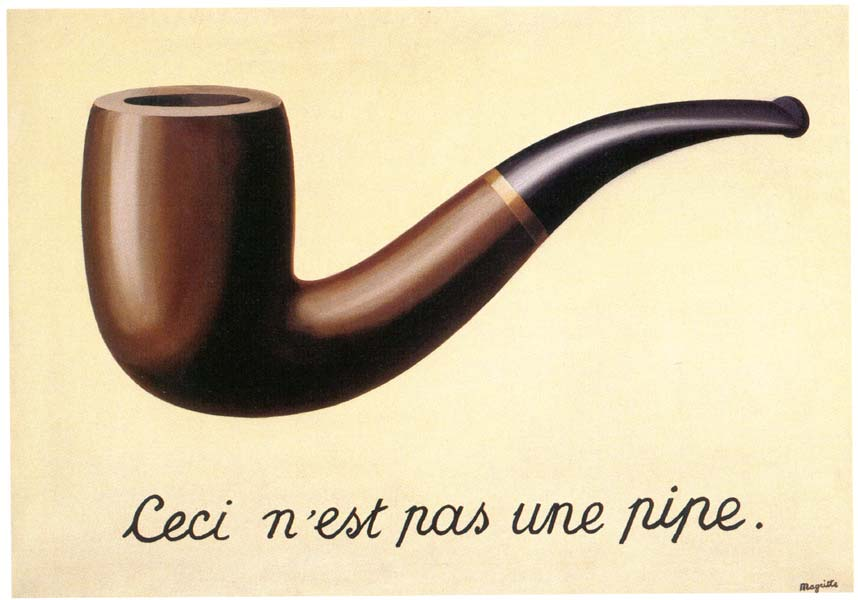
\includegraphics[width=0.8\textwidth]{assets/magritte-pipe.jpg}
    \caption{René Magritte, 1929, \emph{La Trahison des Images} o \emph{Ceci n'est
      pas une pipe}}
  \end{figure}
\end{frame}

\subsection{Studenti cooperativi}
\begin{frame}{Studenti cooperativi}
  \begin{itemize}
    \item<1-> condividono appunti, sbobinature, prove vecchie risolte
    \item<2-> non c'è bisogno di proteggere i propri beni: chiunque ha accesso a
      una copia!
  \end{itemize}
\end{frame}

\subsection{Studenti cooperativi: esistono davvero!}
\begin{frame}{Studenti cooperativi: esistono davvero!}
  Studenti della laurea triennale in Informatica:
  \href{https://csunibo.github.io/}{\beamergotobutton{CSUnibo}}.
\end{frame}

\subsection{Studenti cooperativi: lo possiamo essere tutti!}
\begin{frame}{Studenti cooperativi: lo possiamo essere tutti!}
  Laboratorio! Chi sa cosa sia una \emph{wiki}?
\end{frame}

\end{document}
